\subsection{Арифметические свойства интеграла Римана}

В данном билете рассматриваются свойства интегрируемости и значения интегралов при проведении арифметических операций над функциями. Лектор подчеркивает, что в отличие от дифференциального исчисления, где производная суммы или произведения находится по алгоритму, в интегральном исчислении ключевым вопросом является само существование (интегрируемость) результирующей функции.

\subsubsection*{1. Линейность интеграла Римана}

Наиболее важным арифметическим свойством является линейность, которая включает в себя возможность вынесения константы и интегрирование суммы функций.

\begin{theorem}[Линейность]
Пусть функции $f(x)$ и $g(x)$ интегрируемы по Риману на отрезке $[a, b]$ ($f, g \in R([a, b])$). Тогда для любых действительных чисел $\alpha, \beta \in \R$ их линейная комбинация $(\alpha f + \beta g)(x)$ также интегрируема на $[a, b]$, причём:
\[ \int\limits_a^b (\alpha f(x) + \beta g(x)) dx = \alpha \int\limits_a^b f(x) dx + \beta \int\limits_a^b g(x) dx \]
\end{theorem}

\begin{tcolorbox}[title=Доказательство, breakable]
Доказательство основано на свойствах пределов интегральных сумм Римана.

1. Составим интегральную сумму Римана для функции $h(x) = \alpha f(x) + \beta g(x)$ при заданном разбиении $P$ и наборе отмеченных точек $\xi$:
\[ \sigma(h, P, \xi) = \sum_{j=1}^n (\alpha f(\xi_j) + \beta g(\xi_j)) \Delta x_j \]

2. Пользуясь правилами работы с конечными суммами, разделим её на две части:
\[ \sigma(h, P, \xi) = \alpha \sum_{j=1}^n f(\xi_j) \Delta x_j + \beta \sum_{j=1}^n g(\xi_j) \Delta x_j = \alpha \sigma(f, P, \xi) + \beta \sigma(g, P, \xi) \]

3. Так как $f, g \in R([a, b])$, то при $\lambda(P) \to 0$ соответствующие интегральные суммы имеют конечные пределы, равные $\int_a^b f(x) dx$ и $\int_a^b g(x) dx$.

4. Согласно теореме об арифметических свойствах пределов (предел линейной комбинации равен линейной комбинации пределов), существует предел левой части:
\[ \lim_{\lambda(P) \to 0} \sigma(h, P, \xi) = \alpha \lim_{\lambda(P) \to 0} \sigma(f, P, \xi) + \beta \lim_{\lambda(P) \to 0} \sigma(g, P, \xi) \]
\[ \lim_{\lambda(P) \to 0} \sigma(h, P, \xi) = \alpha \int\limits_a^b f(x) dx + \beta \int\limits_a^b g(x) dx \]

Существование конечного предела означает, что функция $h(x)$ интегрируема по Риману, и её интеграл равен полученному значению.
\end{tcolorbox}

\subsubsection*{2. Интегрируемость произведения функций}

\begin{theorem}[Об интегрируемости произведения]
Если функции $f(x)$ и $g(x)$ интегрируемы по Риману на отрезке $[a, b]$, то их произведение $f(x) \cdot g(x)$ также интегрируемо по Риману на этом отрезке.
\end{theorem}

\begin{tcolorbox}[title=Доказательство (схема), breakable]
Для доказательства используется критерий Дарбу в терминах колебаний.
1. Так как $f$ и $g$ интегрируемы, они ограничены: $|f(x)| \le M_f, |g(x)| \le M_g$.
2. Колебание произведения на элементарном отрезке $\Delta_j$ оценивается так:
\[ \omega(fg, \Delta_j) \le M_f \omega(g, \Delta_j) + M_g \omega(f, \Delta_j) \]
3. Умножая на $\Delta x_j$ и суммируя, получаем:
\[ \sum \omega(fg, \Delta_j) \Delta x_j \le M_f \sum \omega(g, \Delta_j) \Delta x_j + M_g \sum \omega(f, \Delta_j) \Delta x_j \]
4. Поскольку обе суммы в правой части стремятся к нулю при $\lambda(P) \to 0$ (в силу интегрируемости $f$ и $g$), то и левая часть стремится к нулю. По критерию Дарбу, произведение интегрируемо.
\end{tcolorbox}

\subsubsection*{3. Интегрируемость модуля и частного}

\begin{itemize}
    \item \textbf{Модуль:} Если $f \in R([a, b])$, то $|f| \in R([a, b])$. Это следует из неравенства для колебаний $\omega(|f|, \Delta) \le \omega(f, \Delta)$.
    \item \textbf{Частное:} Если $f, g \in R([a, b])$ и существует такое $c > 0$, что для всех $x \in [a, b]$ выполняется $|g(x)| \ge c$, то частное $f(x)/g(x)$ также интегрируемо на $[a, b]$.
\end{itemize}

\subsubsection*{Геометрический смысл}
Линейность интеграла имеет прозрачную геометрическую интерпретацию:
\begin{enumerate}
    \item Вынесение константы $\alpha$ соответствует «растяжению» фигуры вдоль оси $Oy$ в $\alpha$ раз, что во столько же раз меняет её площадь.
    \item Интеграл суммы соответствует «сложению» высот двух криволинейных трапеций. Суммарная площадь под графиком $f+g$ равна сумме площадей под каждым графиком в отдельности.
\end{enumerate}

%\begin{center}
%\includegraphics[width=0.6\textwidth]{linearity_geometry.png}
% На рисунке должны быть изображены два графика f(x) и g(x), 
% а также их сумма (f+g)(x). Заштрихованные области под f и g 
% в сумме дают площадь области под графиком суммы.
%\end{center}

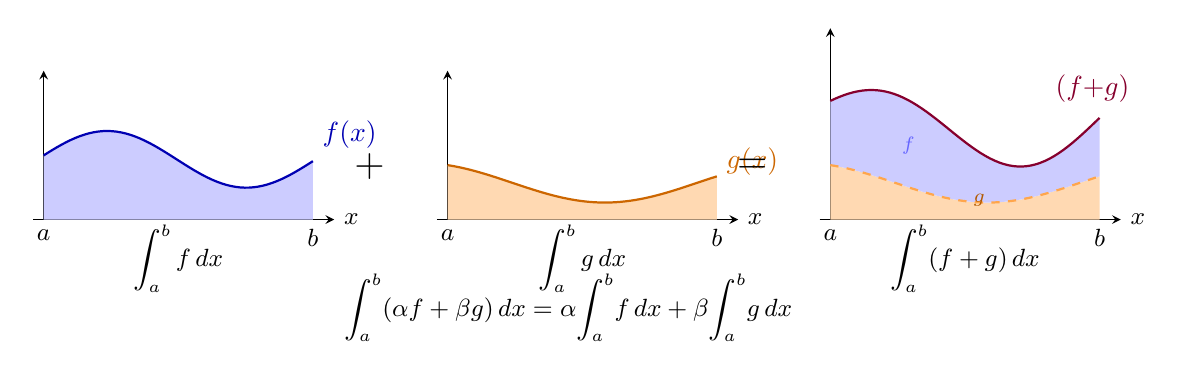
\begin{tikzpicture}[>=stealth, scale=0.9]
 
\def\xa{0.4}
\def\xb{4.2}
 
%==== (1) f(x) ====
\begin{scope}[xshift=0cm]
  \draw[->,thin] (\xa-0.15,0)--(\xb+0.3,0) node[right,font=\small]{$x$};
  \draw[->,thin] (\xa,0)--(\xa,2.1);
  \fill[blue!20,domain=\xa:\xb,samples=60]
    plot(\x,{0.4*sin(deg(\x*1.6-0.5))+0.85})
    -- (\xb,0) -- (\xa,0) -- cycle;
  \draw[blue!70!black,thick,domain=\xa:\xb,samples=60]
    plot(\x,{0.4*sin(deg(\x*1.6-0.5))+0.85});
  \node[blue!70!black,font=\itshape,right] at (\xb,1.2){$f(x)$};
  \node[below,font=\small] at (\xa,0){$a$};
  \node[below,font=\small] at (\xb,0){$b$};
  \node[font=\small] at (2.3,-0.55){$\displaystyle\int_a^b f\,dx$};
\end{scope}
 
\node[font=\Large] at (5.0,0.75){$+$};
 
%==== (2) g(x) ====
\begin{scope}[xshift=5.7cm]
  \draw[->,thin] (\xa-0.15,0)--(\xb+0.3,0) node[right,font=\small]{$x$};
  \draw[->,thin] (\xa,0)--(\xa,2.1);
  \fill[orange!30,domain=\xa:\xb,samples=60]
    plot(\x,{0.28*cos(deg(\x*1.2))+0.52})
    -- (\xb,0) -- (\xa,0) -- cycle;
  \draw[orange!80!black,thick,domain=\xa:\xb,samples=60]
    plot(\x,{0.28*cos(deg(\x*1.2))+0.52});
  \node[orange!80!black,font=\itshape,right] at (\xb,0.82){$g(x)$};
  \node[below,font=\small] at (\xa,0){$a$};
  \node[below,font=\small] at (\xb,0){$b$};
  \node[font=\small] at (2.3,-0.55){$\displaystyle\int_a^b g\,dx$};
\end{scope}
 
\node[font=\Large] at (10.4,0.75){$=$};
 
%==== (3) f(x)+g(x) ====
\begin{scope}[xshift=11.1cm]
  \draw[->,thin] (\xa-0.15,0)--(\xb+0.3,0) node[right,font=\small]{$x$};
  \draw[->,thin] (\xa,0)--(\xa,2.7);
  % нижний слой — g
  \fill[orange!30,domain=\xa:\xb,samples=60]
    plot(\x,{0.28*cos(deg(\x*1.2))+0.52})
    -- (\xb,0) -- (\xa,0) -- cycle;
  % верхний слой — f поверх g
  \fill[blue!20,domain=\xa:\xb,samples=60]
    plot(\x,{(0.4*sin(deg(\x*1.6-0.5))+0.85)+(0.28*cos(deg(\x*1.2))+0.52)})
    -- (\xb,{0.28*cos(deg(\xb*1.2))+0.52})
    -- plot[domain=\xb:\xa,samples=60]
         (\x,{0.28*cos(deg(\x*1.2))+0.52})
    -- cycle;
  % кривая f+g
  \draw[purple!70!black,thick,domain=\xa:\xb,samples=60]
    plot(\x,{(0.4*sin(deg(\x*1.6-0.5))+0.85)
             +(0.28*cos(deg(\x*1.2))+0.52)});
  % граница g (пунктир)
  \draw[orange!70,dashed,thick,domain=\xa:\xb,samples=60]
    plot(\x,{0.28*cos(deg(\x*1.2))+0.52});
  \node[purple!70!black,font=\itshape] at (\xb-0.1,1.85){$(f{+}g)$};
  \node[below,font=\small] at (\xa,0){$a$};
  \node[below,font=\small] at (\xb,0){$b$};
  % метки слоёв
  \node[font=\scriptsize,orange!70!black] at (2.5,0.28){$g$};
  \node[font=\scriptsize,blue!60] at (1.5,1.05){$f$};
  \node[font=\small] at (2.3,-0.55){$\displaystyle\int_a^b(f+g)\,dx$};
\end{scope}
 
% общая формула
\node[font=\small] at (7.8,-1.25)
  {$\displaystyle\int_a^b(\alpha f+\beta g)\,dx
    =\alpha\!\int_a^b\!f\,dx+\beta\!\int_a^b\!g\,dx$};
 
\end{tikzpicture}